
\documentclass[utf8]{ctexart}
\usepackage{booktabs}
\usepackage{tikz}
\usepackage{geometry}
\usepackage{enumerate}
\usepackage{makecell}
\geometry{left=2.0cm,right=2.0cm,top=2.5cm,bottom=2.5cm}
\begin{document}

\begin{bfseries} 
 电池测试系统项目开发执行书
\end{bfseries}

\section {模型实验安排}
项目模型打开方法:mt charge

项目源码打开方法:kl charge

项目设计打开方法:la charge (本设计文档)

设计模型 -> 

\section {气缸控制实现}
\subsection {控制环境}
\begin{enumerate} [1.]
  \setlength{\itemsep}{0.1ex} %条目间距
  \setlength{\itemindent}{2em} %标签缩进量
  \item  OK和NG信号:我的OK端出是多少V时,总系统认为测试OK;我的NG端出是多少V时,总系统认为测试NG;   
  \item  就位信号:测试品就位好时,输出的信号电压是多少V给我的系统?
  \item 气缸参数:给气缸供电24V,它是进还是退, 气缸的型号是什么?有没用到气缸传感器?
     \begin{table}[!htbp]
	    \centering
	    \begin{tabular}{|p{4cm}|p{3cm}|p{7cm}|}
	      \Xhline{1.0pt}
	    站位&气缸编号&气缸作用\\  \Xhline{1.0pt}
	    	电压测试站1&&\\ \hline
	    	电压测试站1&&\\ \hline
	    	电压测试站1&&\\ \hline
		电压测试站1&&\\ \Xhline{1.0pt} 

	    	电压测试站2&&\\ \hline
	    	电压测试站2&&\\ \hline
	    	电压测试站2&&\\ \hline
		电压测试站2&&\\ \Xhline{1.0pt}

	    	电流测试站&&\\ \hline
	    	电流测试站&&\\ \hline
	    	电流测试站&&\\ \hline
		电流测试站&&\\  \Xhline{1.0pt}
	    \end{tabular}
	    \caption{气缸分配表}
    \end{table}
     

\end{enumerate}
\subsection {控制方案} 
     \begin{table}[!htbp]
	    \centering
	    \begin{tabular}{ccclc} \Xhline{1.0pt}
		    分类&数量&作用&技术条件\\ 
		     \Xhline{1.0pt} 
		    气缸通断&2&纵向位移/横向开机&3.3V驱动MOSFET再驱动24V继电器 \\
		    气缸通断&8&纵向位移/横向开机-加减档 &3.3V驱动MOSFET再驱动24V继电器 \\
		    产品短路&1&输出短路电流测试&3.3V驱动MOSFET再驱动24V双刀继电器 \\
		    AC输入&3&测试前后断开 &3.3V驱动MOSFET再驱动24V双刀继电器\\
		    DC输入&3&灵活控制产品充/断电 &3.3V驱动MOSFET再驱动24V双刀继电器 \\
		    信号就位&3&系统开始测试的输入信号&Input\_24V --> Output\_3.3V \\
		    信号OK&3&测试结果的输出信号&Input\_3.3V --> Output\_24V \\
		    信号NG&3&测试结果的输出信号&Input\_3.3V --> Output\_24V \\
		    产品输出&3&电池产品输出分压ADC检测&24AWG导线 \\
		   \Xhline{1.0pt}

	\end{tabular}
	\caption{GPIO引脚按控制功能分配方案}
     \end{table}

电流站:\\1GPIO控制OK信号的输出;1GPIO控制NG信号的输出;1GPIO检测产品就位信号输入,共3个GPIO。\\ 2GPIO控制气缸;1GPIO控制制AC的通断;1GPIO控制DC的通断;1GPIO控制产品短路,共5个GPIO。 

电压站:\\1GPIO控制OK信号的输出;1GPIO控制NG信号的输出;1GPIO检测产品就位信号输入,共3个GPIO。\\ 4GPIO控制气缸;1GPIO控制制AC的通断;1GPIO控制DC的通断;共6个GPIO。

统计:信号用GPIO = 3*3 =9个。\\电力用GPIO = 5 + 6*2 = 17个。\\ 注:电力用意为GPIO驱动MOSFETG来控制24V的供给;“AC/DC/产品短路”的通断采用有MOSFET的24V再控制双联继电器实现AC/DC的双线同时通断。

\subsection {面向对象方法使用}
为改善面向过程的编程方法造成的思路不清晰,及改一处而变全部的弊端,采用面向对象的方法。一个气缸为一个实例,它的执行过程中,会初始化一个新的气缸实例或继电器示例,使这些实例能用指定的变量参数初始化及受控。

构建继电器类,它包含的成员有:施控的GPIO端口、它的施控时间、施控执行函数。这个执行函数可以在控制过程中可以产生、控制其它的继电器实例。

定义抽象类:
Station --- 测试站 它的方法有开始/停止/输出失败/输出成功;它的字段有错误状态值
Relay	--- 继电器 它的方法有ON/OFF/TimeOver;它的字段有名字(得知其功能)、有时间(启动其内部的定时器使其Relay反转)、初始状态(默认ON还是OFF);

定义类:
Relay_air	--- 气缸用继电器,
Relay_short

实例:
原则是每个执行部件都是一个实例。这些实例,在station实例进入工作状态时,被逐次激活。当station测试成功、或失败改为还原为初始状态。所以每个实例可能有不同的初始化状态(初始化时用参数控制)

\subsection {RTOS使用}
\subsection {检测准备好信号, 并用LED提示}

\section {模型设计标准}

\subsection{单支气缸}
单支气缸的动作原理:气缸的动作控制信号只有一个,即通过一个GPIO脚控制气缸电源电压的通断。但在程序内部(simulink模型中)通过简单改变一个变量求反就可以控制GPIO的翻转。但是控制变量翻转后,会通过一系列的逻辑判断才会确定GPIO是否翻转。

如果GPIO控制的气缸未翻转成功,则会有一个错误代码输出来告知系统出现故障。故障排除后,重置气缸状态(变量初值控制)开始新一轮测试$\footnote{另外章节详细描述的细节}$。

优点是:控制时不用管气缸的当前状态,只是由当前测试程序运行的进度连续施控即可,如果有气缸运行的逻辑错误,会导至测试失败而停止,而不会导致整个运行的错乱。

缺点是:必须确定好气缸的初始状态,也许中途会异想不到的气缸上下逻辑错位。

\begin{figure}[htbp]
\centering
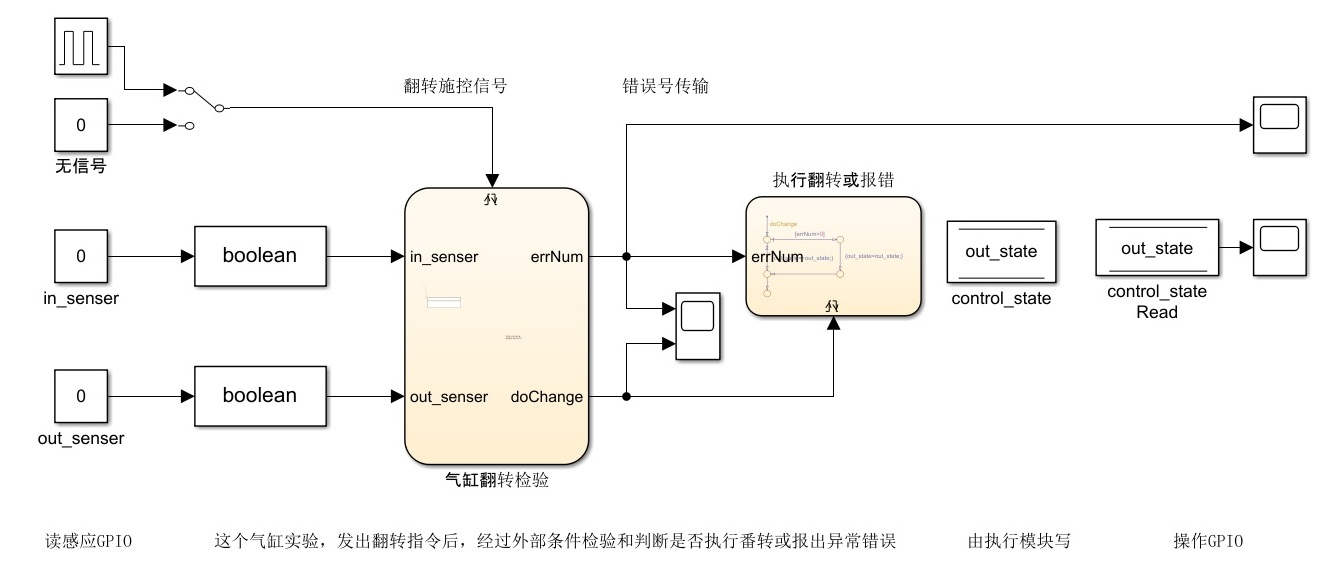
\includegraphics[height=8.0cm,width=15cm]{imgs/dqg.jpg}
\caption{单气缸控制模型}
\end{figure}

气缸执行错误代码,当多组多气缸时再对错误代码进行扩展编制, 让系统识别是哪组及哪个气缸的异常。
\begin{table}[!htbp]
	\centering
	\begin{tabular}{cccc}
	%\multicolumn{4}{|c|}{变量表}\\ % 合并三列 居中,两边加线
	\toprule
	错误代号&错误说明&原因\\  \hline
		2&两气缸位置传感器同时为ON&可能传感器故障\\
		1&气缸位置传感器信号与控制状态(out\_state)不一值&可能传感器接反\\
		0&没有错误&正常情况\\
		-2&两气缸位置传感器同时为OFF&可能传感器故障,或未采用传感系统\\
	\bottomrule
	\end{tabular}
	\caption{错误代码表}
\end{table}


\subsection{一站气缸组}
各电流测试或电压测试站,可能会有多于一个或两个的气缸完成行程和开机及调档。这些气缸要按照预定的顺序动作,动作时序是通过产生的一序列信号来同步。

联动分析:被测品就位,第一气缸纵向传送探针到与产品按钮水平位置;再由第二气缸模向传送探针到产品输出;其它气缸控制开机或调档的按钮。

每个气缸动作都会由\underline{\hbox to 1.5cm{}}        开始,由\underline{\hbox to 1.5cm{}}     结束。有的气缸会在前一个气缸动作完后动作,而有些气缸会同时动作。所以气缸组的联动关键是设计联动信号组,为了能灵活变动及组合,最好设计成动态变量分配控制形式。

由表2的定义,可以让程序查表为初始化程序。每次气缸做不同的动作会有不同的时间限制。这个表可由电脑修改,灵活方便定义程序初始化状态。(将要实现数据同步模型)

\begin{table}[!htbp]
	\centering
	\begin{tabular}{c|c|cc|c}
		\toprule
		气缸代号&名称&初始状态变量&值&气缸用途 \\ \hline
		P1S1&站位1气缸1&act\_sta&0(抬起)&移动按建器 \\
		P1S2&站位1气缸2&act\_sta&0(抬起)&上下就位键 \\
		P1S3&站位1气缸2&act\_sta&0(抬起)&其它 \\
		\bottomrule
	\end{tabular}
	\caption{电流测试站气缸状态初始表}
\end{table} 
注· 这个表的值是可变的,将会被电脑程序更改。若要更改或查看实际设定值的方法是:~~~~

\begin{table}[!htbp]
	\centering
	\begin{tabular}{c|c|cc|cc|c}
		\toprule
		联动顺序&气缸代号&动作变量&值&计时变量&值&动作说明 \\ \hline
		1&P1S1&act\_sta&0(抬起)&act\_tim&25(ms)&移动按建器 \\
		2&P1S2&act\_sta&0(抬起)&act\_tim&25(ms)&执行按键器1次 \\
		3&P1S3&act\_sta&0(抬起)&act\_tim&25(ms)&回退按键器1次 \\
		\bottomrule
	\end{tabular}
	\caption{电流测试站气缸动作时序表}
\end{table} 


\subsection{多站式气缸群}
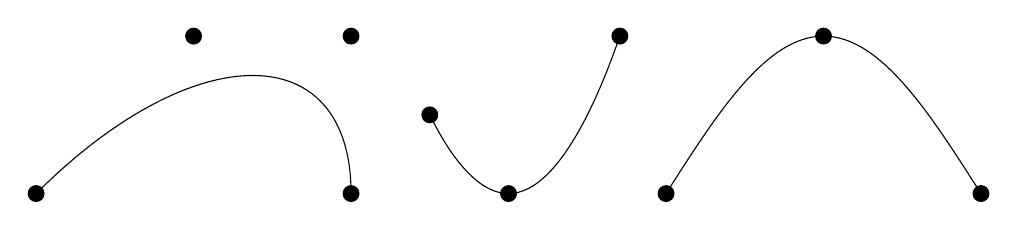
\begin{tikzpicture}
     \draw (0,0)..controls (2,2) and (4,2)..(4,0);
     \filldraw (0,0) circle (.1) (2,2) circle (.1) (4,2) circle (.1) (4,0) circle (.1);
     \draw (5,1) parabola bend (6,0) (7.414,2);
     \filldraw (5,1) circle (.1) (6,0) circle (.1) (7.414,2) circle (.1);
     \draw (8,0) sin (10,2) cos (12,0);
     \filldraw (8,0) circle (.1) (10,2) circle (.1) (12,0) circle (.1);
\end{tikzpicture}
\end{document}
